\documentclass[12pt,preprint]{aastex}

\usepackage{latexsym}
\usepackage{fancybox}
\usepackage{graphicx}
\usepackage{amssymb}
\usepackage{color}
\usepackage{ulem}
\usepackage{float}
\usepackage{multicol}
\usepackage{enumitem}
\usepackage[hidelinks]{hyperref}
%\usepackage{setspace}
\usepackage{xcolor}  % for the links
\hypersetup{
    colorlinks,
    linkcolor={red!50!black},
    citecolor={blue!50!black},
    urlcolor={blue!80!black}
}

\pretolerance=10000
\textwidth=6.5in
\textheight=9.2in
\voffset = 0.0in
\topmargin=0.0in
\headheight=0.00in
\hoffset = 0.0in
\headsep=0.20in
\oddsidemargin=0in
\evensidemargin=0in
\parindent=2em
\parskip=0.25ex
 
%\input{defs_xavier}
%\input{/u/xavier/bin/latex}
%\input{/u/xavier/bin/defs}

\newcommand{\npair}{50}
\def\ssp{\def\baselinestretch{1.0}\large\normalsize}
\newcommand{\oneskip}{\vskip \baselineskip}
\newcommand{\annrev}{ARA\&A}
\newcommand{\za}{z$_{ abs}$}
\newcommand{\zg}{z$_{ galaxy}$}
\newcommand{\zl}{$z_{emitter}$}
\newcommand{\zf}{z$_{df}$}
\newcommand{\avxi}{$\langle\xi\rangle$}
\newcommand{\omg}{$\Omega_{g}(z)$}
\newcommand{\tu}{$\tau( > M)$}
\newcommand{\mc}{$10^{12}M_{\odot}$}
\def \lnhi {$\log N_{HI}$}
\def \cmm  {cm$^{-2}$}
\def \cmmm {cm$^{-3}$}
\def \hfreq {$f_{\rm{HI}} (N,X)$}
\def \gamrate {$\Gamma_{912}$}
\def \fn {$f_{\rm{HI}} (N,X)$}
\def \lyaf {Ly--$\alpha$ forest}
\def \nqso  {seven}
\def \cmm  {\rm cm^{-2}}
\newcommand{\lya}{Ly$\alpha$}

\usepackage{multicol}

\newenvironment{my_itemize}{
\begin{itemize}
  \setlength{\itemsep}{1pt}
  \setlength{\parskip}{0pt}
  \setlength{\parsep}{0pt}}{\end{itemize}
}

\newenvironment{my_enumerate}{
\begin{enumerate}
  \setlength{\itemsep}{1pt}
  \setlength{\parskip}{0pt}
  \setlength{\parsep}{0pt}}{\end{enumerate}
}



\usepackage{geometry}
\geometry{letterpaper,tmargin=1.3in,bmargin=0.7in,lmargin=0.95in,rmargin=0.95in}
\usepackage[layout=modern]{advancedcoverpage}


\title{{\Large PypeIt:  A Data Reduction Pipeline for UCO and WMKO}}

\presentedto{{\large \underline{2018 UCO Call for mini-grants}} \\
\vskip 0.1in
{\it Submitted to the UCOAC}
}


\author{
{\bf PI:} 
J. Xavier Prochaska (UCSC) \\
\vskip 0.1in
{\bf UC Faculty/Staff/PhD Co-I's:} \\
Joseph F. Hennawi (UCSB) \\
Kyle Westphal (UCO) \\
Tiffany Hsyu (UCSC) \\
Lawrence Lawson (UCSC) \\
%Carl Melis (UCSD) \\
\vskip 0.1in
\vskip 0.1in
{\bf other Co-I's:} \\
R. Cooke (Durham), Luca Rizzi (WMKO) \\
\vskip 0.3in
%\includegraphics[width=5.5in]{../WhitePaper/title_fig2.pdf}
{\bf Abstract:} \\
We request a UCO mini-grant to fund the continued development of PypeIt,
an open source python based data reduction pipeline for echelle, longslit, and multi-slit
observations on UCO optical and near-IR spectrometers.
This project is being pursued in collaboration with WMKO,
following the recommendation of the Keck SSC.
To meet UCO's commitment and expand the capability
to other UCO facility instruments, we require the
funding requested within.
}

 
\begin{document}
\maketitle

	\pagestyle{myheadings}    % Go for customized headings
%\markright{Prochaska--U079 2008A Proposal---Quasars Probing Quasars}
	\markboth{\hfill Prochaska -- PypeIt (v1.0) \hfill}{\hfill
          Prochaska -- PypeIt (v1.0) \hfill}



%%%%%%%%%%%%%%%%%%%%%%%%%%%%%%%%%%%%%%%%%%%%%%%%%%%%%%%%%%%%%
%\vskip 0.2in

\noindent {\bf Introduction:} For the past several years, we have been developing a Python
based data reduction pipeline (DRP) named PypeIt\footnote{
Formerly PYPIT;
\href{https://github.com/pypeit/PypeIt}{PypeIt github repository};
\href{http://pypeit.readthedocs.io/en/latest/}{PypeIt docs}}.
While driven initially and primarily by our own scientific
needs, we designed and built the PypeIt architecture
with several guiding philosophies that enable it to be used more generally:

\vskip -0.2in

\begin{my_itemize}
\item Python (3.6 or greater)
\item Implement modern practices for shared code development 
(i.e.\ git, github)
\item Encourage community usage and contributions
\item Include minimal dependencies (emphasis on numpy, scipy, astropy)
\item Construct unit tests and data
\href{https://github.com/pypeit/PypeIt-development-suite}{test suites}
with 
\href{https://travis-ci.org/PypeIt/PypeIt/}{continuous integration}
\item Integrate with WMKO and the broader community (e.g.\ {\it astropy})
\end{my_itemize}

\vskip -0.1in

\noindent
In April 2017, we released v0.2 of PypeIt which included 
support for Keck/LRIS and Lick/Kast. 
%, and echelle spectrometers(APF, HIRES).
In Spring/Summer 2017, we were invited to participate
in the WMKO-led Data Reduction Working Group (DRWG). We 
\href{https://www.dropbox.com/s/n17il1aah1xs6fx/ucsc_PypeIt_mar2017.pdf?dl=0}
{presented} to that group our progress with PypeIt and
lessons learned from our 18+ years of DRP development in 
IDL. %\footnote{
%\href{http://www.ucolick.org/~xavier/LowRedux/}{LowRedux};
%\href{http://www.ucolick.org/~xavier/HIRedux/}{HIRedux}
%}.
We helped develop the recommendations of the DRWG as 
presented\footnote{\href{https://www.dropbox.com/s/k7ykp80voslaw7o/DRWG_June2017_SSC_v2.pptx?dl=0}{DRWG presentation}} 
to the Keck/SSC.  This presentation was well received by the
SSC, which recommended that we present a detailed development plan and a well defined set of requirements for DRP development.  
We have completed the majority of that work.
Figure~\ref{fig:DEIMOS_example} shows
the near Poisson-limit data reduction of DEIMOS
multi-slit spectra.

In September 2018, we released v0.9 for beta testing of 
the LRIS, DEIMOS,
NIRES, NIRSPEC, and Kast instruments.
We plan to release v1.0 on 1/1/2019 to the full community.
As FY19 begins for WMKO,
we have agreed to spend Year~2 expanding PypeIt to include
the ESI, HIRES, MOSFIRE, and KCWI instruments at WMKO.
%that supports all Longslit modes of Keck/LRIS (save polarimetry)
%in a more modularized version of PypeIt, as well developing the
%tools for full Multi-slit support. It is planned that this
%will lay the foundation for all other future development of
%spectroscopic DRPs at WMKO.
This proposal to the mini-grant process will fund
that activity at UCO (and elsewhere) while staff at WMKO
focus on 
[LUCA FILLS IN HERE]
%updating the observing infrastructure to produce complete metadata (slitmask design software, instrument configuration manager and observations execution tools).%\footnote{WMKO requested additional
%resources for DRP development at IPAC in the NASA overguide.
%That proposal was well received but not funded.  We expect they
%will reapply in 2018.}


%%%%%%%%%%%%%%%%%%%%%%%%%
%%%%%%%%%%%%%%%%%%%%%%%%%
%\vskip 0.1in

\noindent 
{\bf Nuts and Bolts:} 
The requested funding from this mini-grant will support
several developments in PypeIt that will benefit the UC
community.  We describe each in turn and summarize the
timeline in Table~\ref{tab:timeline} and Figure~\ref{fig:PypeIt}.
We further emphasize that PypeIt is not a stand-alone,
two-year project;
the UCOAC should recommend to the Director that
a `permanent' line of funding be allocated to this
project, in coordination with WMKO.
It is not the intent of the PI to propose for this
program again.


%%%%%%%%%%%%%%%%%%%%%%%%%
%\vskip -0.15in

\noindent 
{\it Core Development:} 
There are three core activities for PypeIt that demand the
skill set and focused dedication of a staff programmer
in UCO's Scientific Programming Group (SPG):

\vskip -0.15in

\begin{my_enumerate}

\vskip -0.15in

\item  Port the existing KCWI DRP (at least the geometric
mappings) from IDL into PypeIt.  This may require 
input from the lead author (D. Neil) although we will 
perform most of the work independently.
We will consult with the KCRM team to insure the development
coincides with their needs.  We estimate 2 months of 
time to complete this work.

\item XXX???

\item Parallelize the code, where possible.  The obvious drawback
of coding in Python is performance and PypeIt suffers accordingly.
There are, however, several tasks which may be parallelized
for standard multi-core platforms using {\tt map/pool} methods.
We estimate 1.5~months of SPG effort to begin this work, 
focusing on the areas which would provide greatest 
improvement in computational time (e.g.\ sky subtraction). 
%(in particular, the routines for object/sky 
%boundary definition, sky subtraction, optimal extraction).
\end{my_enumerate}

\vskip -0.15in

\noindent
All three activities demand a professional programmer
and we request 0.5~FTE of SPG support at UCO where
the staff member can interact directly with PI Prochaska.
We are hoping that Dr.\ Westphal who joined the project
last year can continue in this capacity.

%%%%%%%%%%%%%%%%%%%%%%%%%
%\vskip -0.05in
\noindent 
{\it HIRES:} 
Co-I Hennawi, who co-developed and maintains 
IDL-based DRPs for WMKO and UCO, will develop PypeIt 
for echelle observations with Keck/HIRES.
This builds upon Prof.\ Hennawi's previous efforts
with the IDL ESI pipeline. The groundwork for reducing
multi-order echelle data exists in v0.9 of PypeIt, but
wavelength solutions and tools for combining orders are not 
yet complete. 
We request one quarter of teaching buyout for 
him to complete this work and also work on ESI (below). 


%%%%%%%%%%%%%%%%%%%%%%%%%
\vskip 0.05in

\noindent 
{\it ESI:} 
Following on the heels of HIRES, we will extend the
echelle algorithms to work with ESI.  This will require
wavelength algorithms tuned to the CuAr, Xe, and Hg 
lamps of ESI.  It will also require a more careful
handling of fringing and scattered light.
Dr.\ Hennawi will lead this effort.

%%%%%%%%%%%%%%%%%%%%%%%%%
\vskip 0.05in

\noindent 
{\it MOSFIRE:}
In v0.9, PypeIt supports the NIRES and NIRSPEC spectrometers
although we are still completing several
key algorithms, e.g.\  ABBA image subtraction,
telluric fluxing.  We will expand PypeIt to include all
modes of MOSFIRE.
This effort will be led by PhD student
T. Hsyu who has previously contributed to PypeIt
(fluxing, coaddition, NIRSPEC).
We request 1~quarter of GSR support for her to 
complete this effort in 2019.  PI Prochaska will co-develop
and closely manage this portion of the project.


%%%%%%%%%%%%%%%%%%%%%%%%%
\vskip 0.05in

\noindent 
{\it APF echelle:}   
The echelle algorithms for HIRES will be transferred
to APF.  The primary code development will be algorithms
to handle the `red devil' scattered light term.
This will be led by Co-I Cooke with contributions
from PI Prochaska.

%%%%%%%%%%%%%%%%%%%%%%%%%
\vskip 0.05in

\noindent 
{\it SPIT integration:}   
PI Prochaska has developed a convolutional neural network (CNN)
to automatically classify Kast spectral image types, i.e.\ the
SPectral Image Typer (\href{https://github.com/pypeit/spit}{SPIT}).
The project has hired an undergraduate student to integrate
the SPIT software into PypeIt.  We request 6 months additional
support for this undergraduate to expand the development to
include all of the spectrometers.

%In $\approx 11$~years of archived
%Lick data, there are 1514 nights when the
%Hamilton echelle was scheduled (3m and CAT nights). 
%The Hamilton has not been used
%on the 3m in nearly 10 months and with the advent of the APF is
%essentially retired. Many of the Hamilton spectra
%were taken to perform RV measurements
%in the search of exoplanets.  Very few of these
%(reduced) spectra, however, are in the public domain.
%Co-I Melis will develop the echelle mode of PypeIt
%to reduce the entire dataset.  He will then provide
%the calibrated spectra in an easily accessible platform
%for the UC community.  We budget 1~mo. of his effort.

%%%%%%%%%%%%%%%%%%%%%%%%%%
\clearpage

\begin{figure}
 \vskip -0.5in
\begin{center}
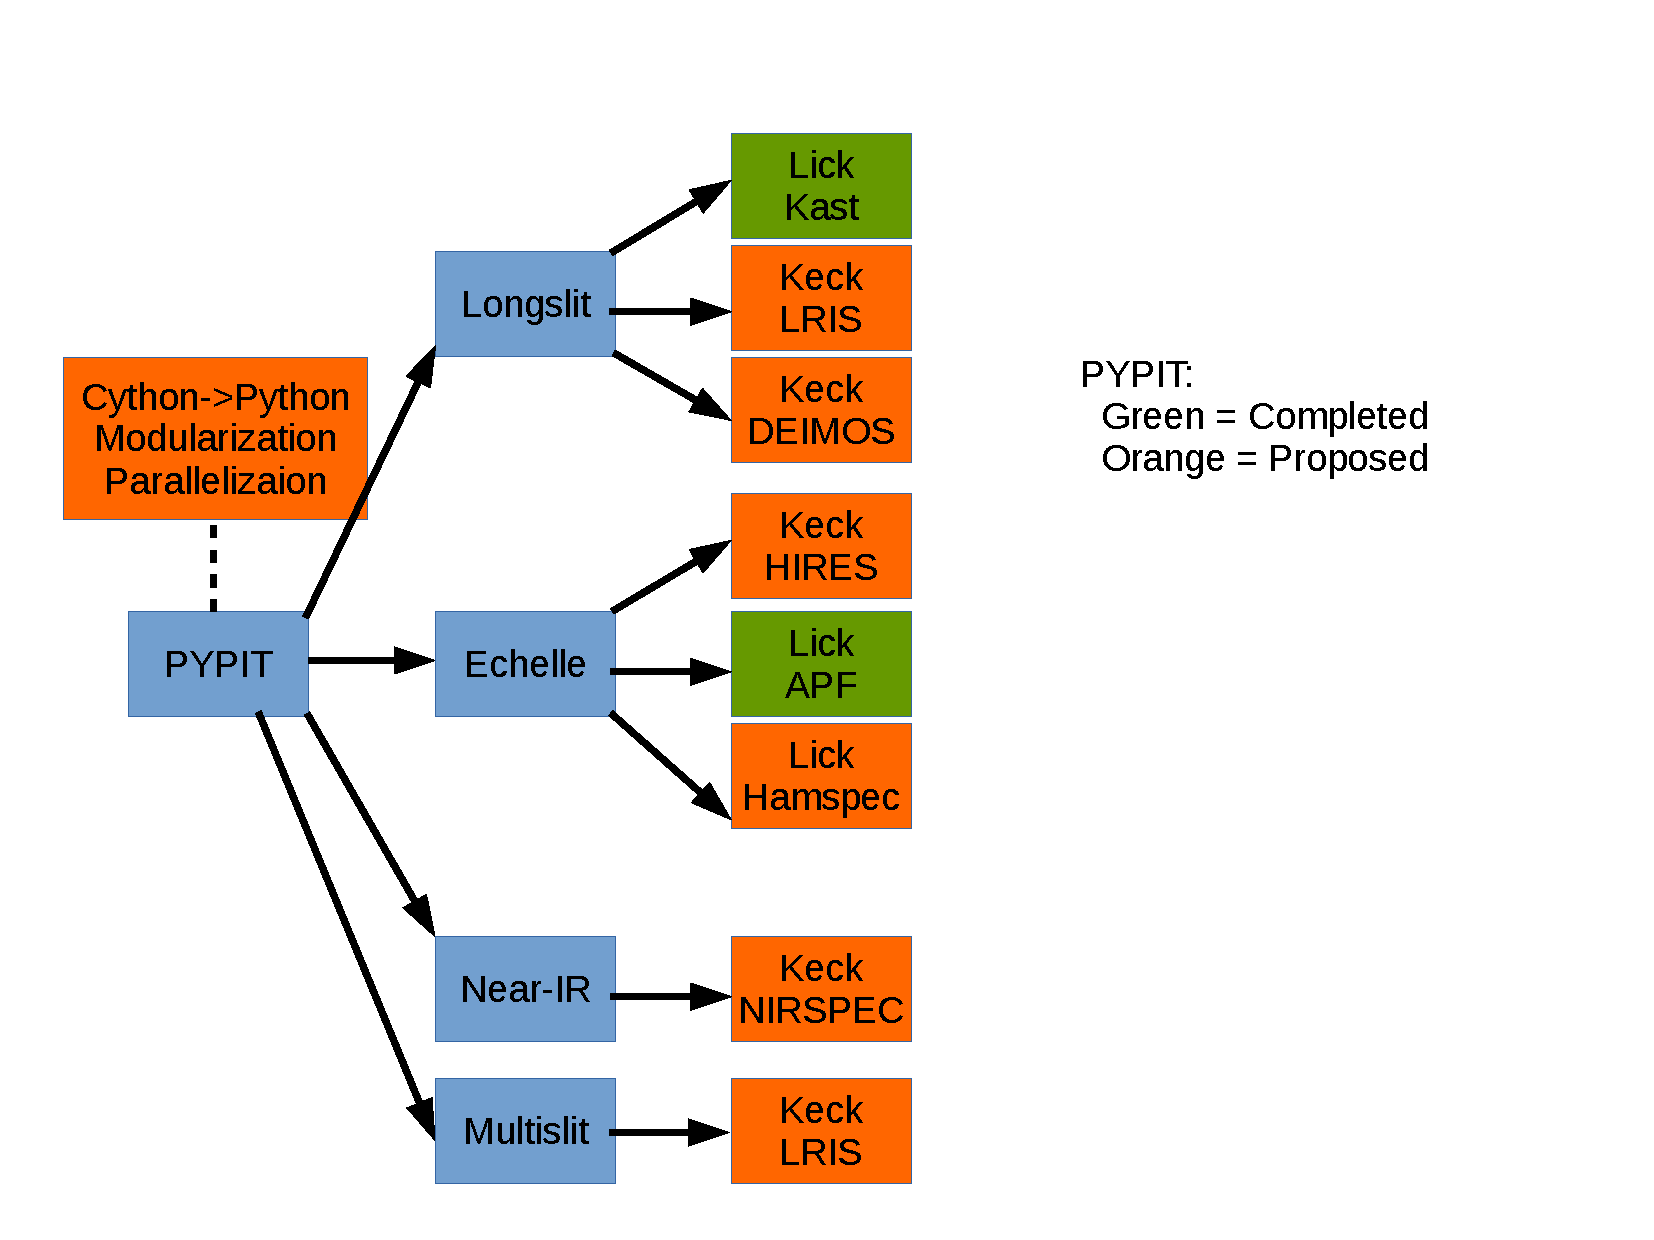
\includegraphics[scale=0.80]{code_sketch.pdf}
\end{center}
 \caption{\footnotesize  
Description of PypeIt as currently implemented (green)
and the proposed development (orange).
}\label{fig:PypeIt}
%  \end{minipage}
\end{figure}

\begin{figure}
 \vskip -0.5in
\begin{center}
%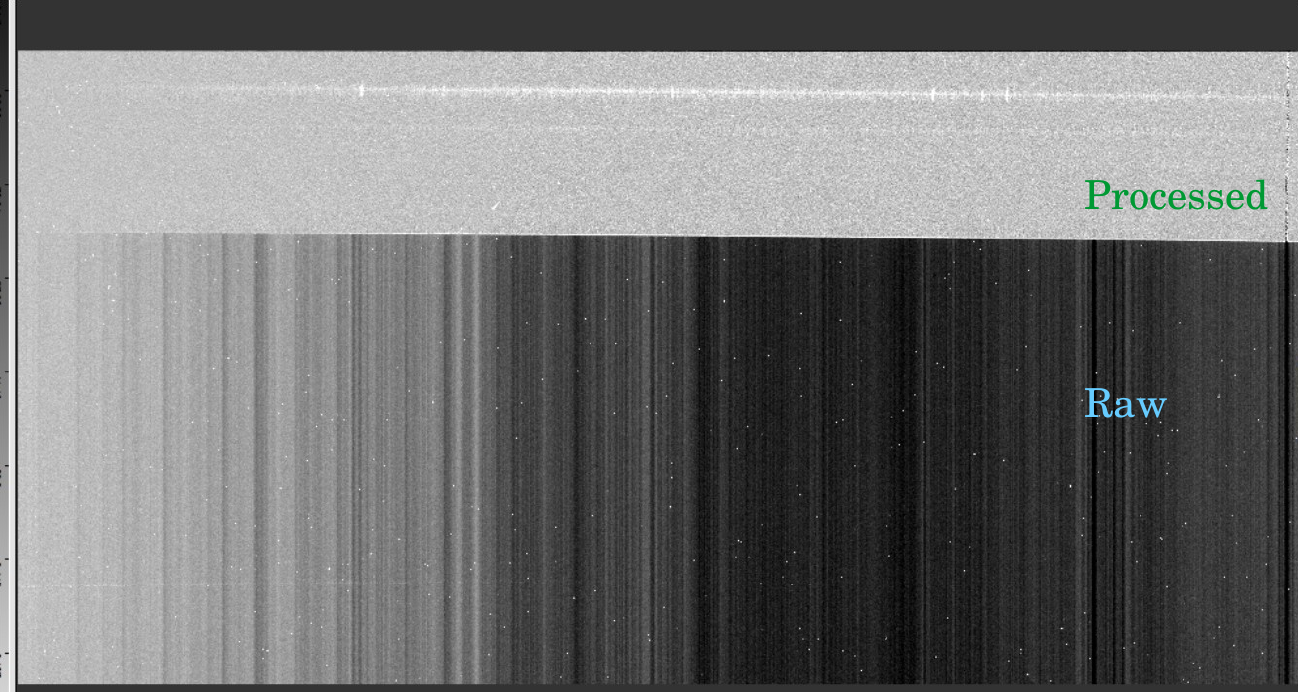
\includegraphics[scale=0.50]{processed_image.png}
\end{center}
 \caption{\footnotesize  
 Need something tasty from Hennawi on DEIMOS
}\label{fig:DEIMOS_example}
%  \end{minipage}
\end{figure}

\clearpage

{\footnotesize

\begin{table}[ht]
\begin{center}
\caption{Timeline \label{tab:timeline}}
\end{center}
\begin{tabular}{lcclccl}
\hline 
Activity & Begin & End & Description & Lead & Effort & Funding \\
\hline 
KCWI & 1/2019 & 6/2019 & Port IDL pipeline & SPG & 2 mo. & \$32,500 \\
%
%Cython $\to$ Python & 1/2018 & 6/2018 & Convert Cython code to Python & SPG & 1.5 mo. & \$24,400 \\
%
Parallelization & 1/2019 & 12/2019 & Implement {\tt map/pool} methods & SPG & 1.5 mo. & \$24,400 \\
%%%%%%%
LRIS/Longslit & 1/2018 & 12/2018 & All modes (save polarimetry) & JXP & 4 mo. & 
\$12,000$^a$ \\
%%%%%%%
HIRES/Echelle & 1/2019 & 12/2019 & All modes & JFH & 2 mo. & \$12,000$^a$ \\
%%%%%%%
ESI/Echelle & 1/2019 & 12/2019 & All modes & JFH & 1 mo. & N/A \\
%%%%%%%
MOSFIRE & 1/2019 & 3/2019 & All modes & TH & 1 qrtr & \$42,175$^b$\\
%%%%%%%
APF & 6/2019 & 9/2019 & Development & JXP & 1 mo. & \$XX,XXX$^c$ \\
%%%%%%%
SPIT & 1/2019 & 6/2019 & Expand usage & LL & 6 mo. & \$XX,XXX$^d$ \\
\hline 
\end{tabular} 
${}^a$ Course relief \\
${}^b$ GSR\\
${}^c$ One month summer-salary\\
${}^d$ Undergrad work-study\\
\end{table} 

}

\noindent
{\bf Salary, Benefits, Course Relief:} \\
The last column of Table 1 describes the costs
for each of the proposed activities.  These total
\$XXX,XXX.
%While the UCOAC may be tempted to 
%consider the above list a `menu', most of the items
%are absolutely critical to the success of the
%project.   
We appreciate the total amount is substantial
but are also aware this is far less than any
serious other DRP effort on a first-class observatory
(e.g.\ {\it HST}, VLT).  \\

\noindent
{\bf Other funding requested:} \\
In addition to the funding covering work effort, we request
\$15,000 in funds to support the travel of Co-I's Hennawi,
Cooke and Rizzi to collaborate at UCO on PypeIt.  This will include
two hack-a-thons (we have held two in 2018).

\end{document}
